\skiptooddpage 
\section{Matroid osztályok}

A következő matroid osztályokat különböztetjük meg: 

\begin{table}[htbp]
\begin{tabular}{|l|ll|}
\hline
Típus& Definició & Példa\\
\hline
\emph{grafikus} & ha egy $G$ gráf által indukált (körmatroid). & $K_3,K_5$ \\
\emph{kografikus} & a grafikus matroidok duálisa. & $K_3,K_5^*$\\
\emph{síkba rajzolható} & ha grafikus $\cap$ kografikus. &$K_3$\\
\emph{reguláris} & ha bármely test felett reprezentálható. & $K_{3,3}^*, K_5 \oplus K_5^*$\\
\emph{bináris} & ha csak a bináris test felett reprezentálható. & $F_7$\\
\emph{lineáris} & ha létezik test amely felett reprezentálható. & $F_7^-$\\
\emph{összes} & ha a korábbiak közül egyik se. & $F_7\oplus F_7^-$\\
\hline
\end{tabular}
\caption{Matroid osztályok}
\end{table}

Ugyanakkor igaz, az osztályokra, hogy grafikus, kografikus $\subseteq$ reguláris
$\subseteq$ bináris $\subseteq$ lineáris $\subseteq$ összes. 


\begin{wrapfigure}{l}{0.35\textwidth}
\caption{A Fano matroid}
\label{fig:Fano}
\centering 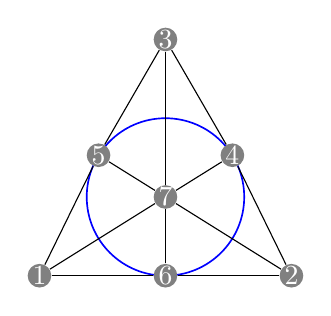
\begin{tikzpicture}[scale=1]
  \tikzset{ p/.style={circle,white,fill=gray,inner sep=0pt,minimum size=0.3cm},
  }
  \draw [semithick,blue] (0,0) circle (1);
  \node[p] (1) at (0.85, 0.53)   {4};
  \node[p] (2) at (0, -1)        {6}; 
  \node[p] (3) at (-1.6 , -1)    {1};
  \node[p] (4) at (-0.85 , 0.53) {5};
  \node[p] (5) at (1.6 , -1)     {2};
  \node[p] (6) at (0 , 2)        {3};
  \node[p] (7) at (0 , 0)        {7};
  
  
  % the connection between the dots
  \draw[-] (1) -- (5); 
  \draw[-] (1) -- (6);
  \draw[-] (1) -- (7);
  
  \draw[-] (2) -- (3);
  \draw[-] (2) -- (5);
  \draw[-] (2) -- (7);
  
  \draw[-] (3) -- (4);
  \draw[-] (3) -- (7);
  
  \draw[-] (4) -- (6);
  \draw[-] (4) -- (7);
  
  \draw[-] (5) -- (7);
  
  \draw[-] (6) -- (7);
\end{tikzpicture} 
\end{wrapfigure}

A Fano matroid egy olyan matroid, amelyben az alaphalmaz mérete $7$ és minden
$2$ elemű részhalmaz független, de minden $3$ elemű csak akkor ha
\aref{fig:Fano} ábrán nincsenek egy körön vagy egy egyenesen. Ha kör megkötést
elhagyjuk az így alkotott matroid az Anti--Fano matroid.

A Fano matroid pontosan azon testek felett reprezentálható amelyek
karakterisztikája $2$ (például a bináris matroid). Az Anti-Fano meg azon testek
felett amelyek karakterisztikája nem kettő. Tehát a két matroid direkt összege
semmilyen test felett nem reprezentálható, azaz nem lineáris.

\vspace{0.4cm}
\emph{Grafikus matroid bármely test felett reprezentálható (reguláris).}
\vspace{0.4cm}

Induljunk ki egy $n$ pontú gráfból, tetszőleges irányitással, rendeljünk minden
ponthoz egy-egy $n$ dimmenziós egységvektort. Az élekhez rendeljük a két
végpontjuk közti különbséget (az irányitás lényegtelen). Azt szeretnénk
bebizonyitani, hogy egy élhalmaz akkor lineárisan független, ha az általa
kifeszített részgráf körmentes.

$\Rightarrow$  Az élek vektorjában csak $0,1$ vagy $-1$ áll, tehát ezek bármely
test felett reprezentálhatóak. Ha a gráfban egy kör menti éleket összeadjuk null vektort
kapunk, mert a megfelelő nem nulla koordináták kiejtik egymást (az összeghez az
élet hozzáadjuk ha kör körbejárási iránya megegyezik az él irányával, és
kivonjuk egyébként -- $1$ vagy $-1$ együtthatók).

$\Leftarrow$ Fordítva, vegyünk egy összefüggő vektorhalmazt és ennek egy olyan X
nemüres részhalmazát amely olyan lineáris kombinációja ad nullát, ahol semelyik
együtható nem nulla. Az élvektor azokon a koordinátákon nem nulla, amelyik
pontokat összeköt. 

Ahhoz, hogy a nullvektor kijöjjön minden ponthoz két darab nem nulla koordináta
kell, hogy létezzen. Azaz egy pontra két él illeszkedik, amely szerint minden
ilyen pont foka nagyobb mint $2$.  Egy adott részgráfban, ahol minden csúcs foka
nagyobb mint kettő, biztosan létezik kör.

\subsection{Tutte tételei}

M matroid $\begin{cases}
\mbox{bináris} &\Leftrightarrow \mbox{ nem tartalmazza minorként: } U_{4,2}. \\ 
\mbox{reguláris} &\Leftrightarrow \mbox{ nem tartalmazza minorként: } U_{4,2}, F_7, F_7^*. \\
\mbox{grafikus} &\Leftrightarrow \mbox{ nem tartalmazza minorként: } \parbox[t]{4cm}{
$U_{4,2},$ $F_7$, $F_7^*$, $M^*(K_5)$, $M^*(K_{3,3})$.} \\
\end{cases}$

\subsection{Seymour tétel}

$M$ reguláris $\Leftrightarrow$  előáll $1$ grafikus, $1$ kografikus és egy
$R_{10}$ matroid példányából a direkt összeg, $2$-összeg és $3$-összeg műveletek
segítségével.

Az $R10$ egy $5$ rangú elem, egy $10$ elemű halmazon: nem grafikus és nem
kografikus.

\begin{figure}[htb]
\caption{Az $R_{10}$}
\label{fig:Seymour}
\centering \begin{tikzpicture}[scale=1]
\matrix [matrix of math nodes,left delimiter={(},right delimiter={)}]
{
1 & 1& 1& 1&  1 & 1 & 0 & 0 & 0 & 0\\
1 & 1& 1& 0 & 0 & 0 & 1 & 1 & 1 & 0\\
1 & 0& 0& 1 & 1 & 0 & 1 & 1 & 0 & 1\\
0 & 1& 0& 1 & 0 & 1 & 1 & 0 & 1 & 1\\
0 & 0& 1& 0 & 1 & 1 & 0 & 1 & 1 & 1\\
};\end{tikzpicture} 
\end{figure} 